\section{Z Bunch Profile Studies}
\label{ch:ZBunchProfileStudies}

\begin{frame}{The Z Bunch Profile}

Last time we discussed directly using the z-bunch profile in the hourglass
simulation. Here I discuss preliminary methods and results

\end{frame}

\begin{frame} {The Z Bunch Profile}
\begin{itemize}
\item Recall that our model of luminosity depends on the convelution of two normal,
three dimensional distriubtions moving through each-other:
\end{itemize}
\begin{equation}
\label{eq:generalluminosity}
\mathcal{L} \propto \iiiint _{\infty}^{ \infty}{
\rho_{blue} (x,y,z-ct_0)\rho_{yellow} (x,y,z+ct_0)} dxdydzdt
\end{equation}
\begin{itemize}
\item And that we may do simple substitutions for coordinates to represent rotations
and $\beta^{*}$ squeezing.

\item We need a means to use a distriubtion of points similarly to a function, so that
we may achieve a mapping of inputs (or transformed inputs) to outputs.
\end{itemize}
\end{frame}

\begin{frame}{The Z Bunch Profile}
We start with the fine-binned profile:
\begin{figure}
\begin{center}
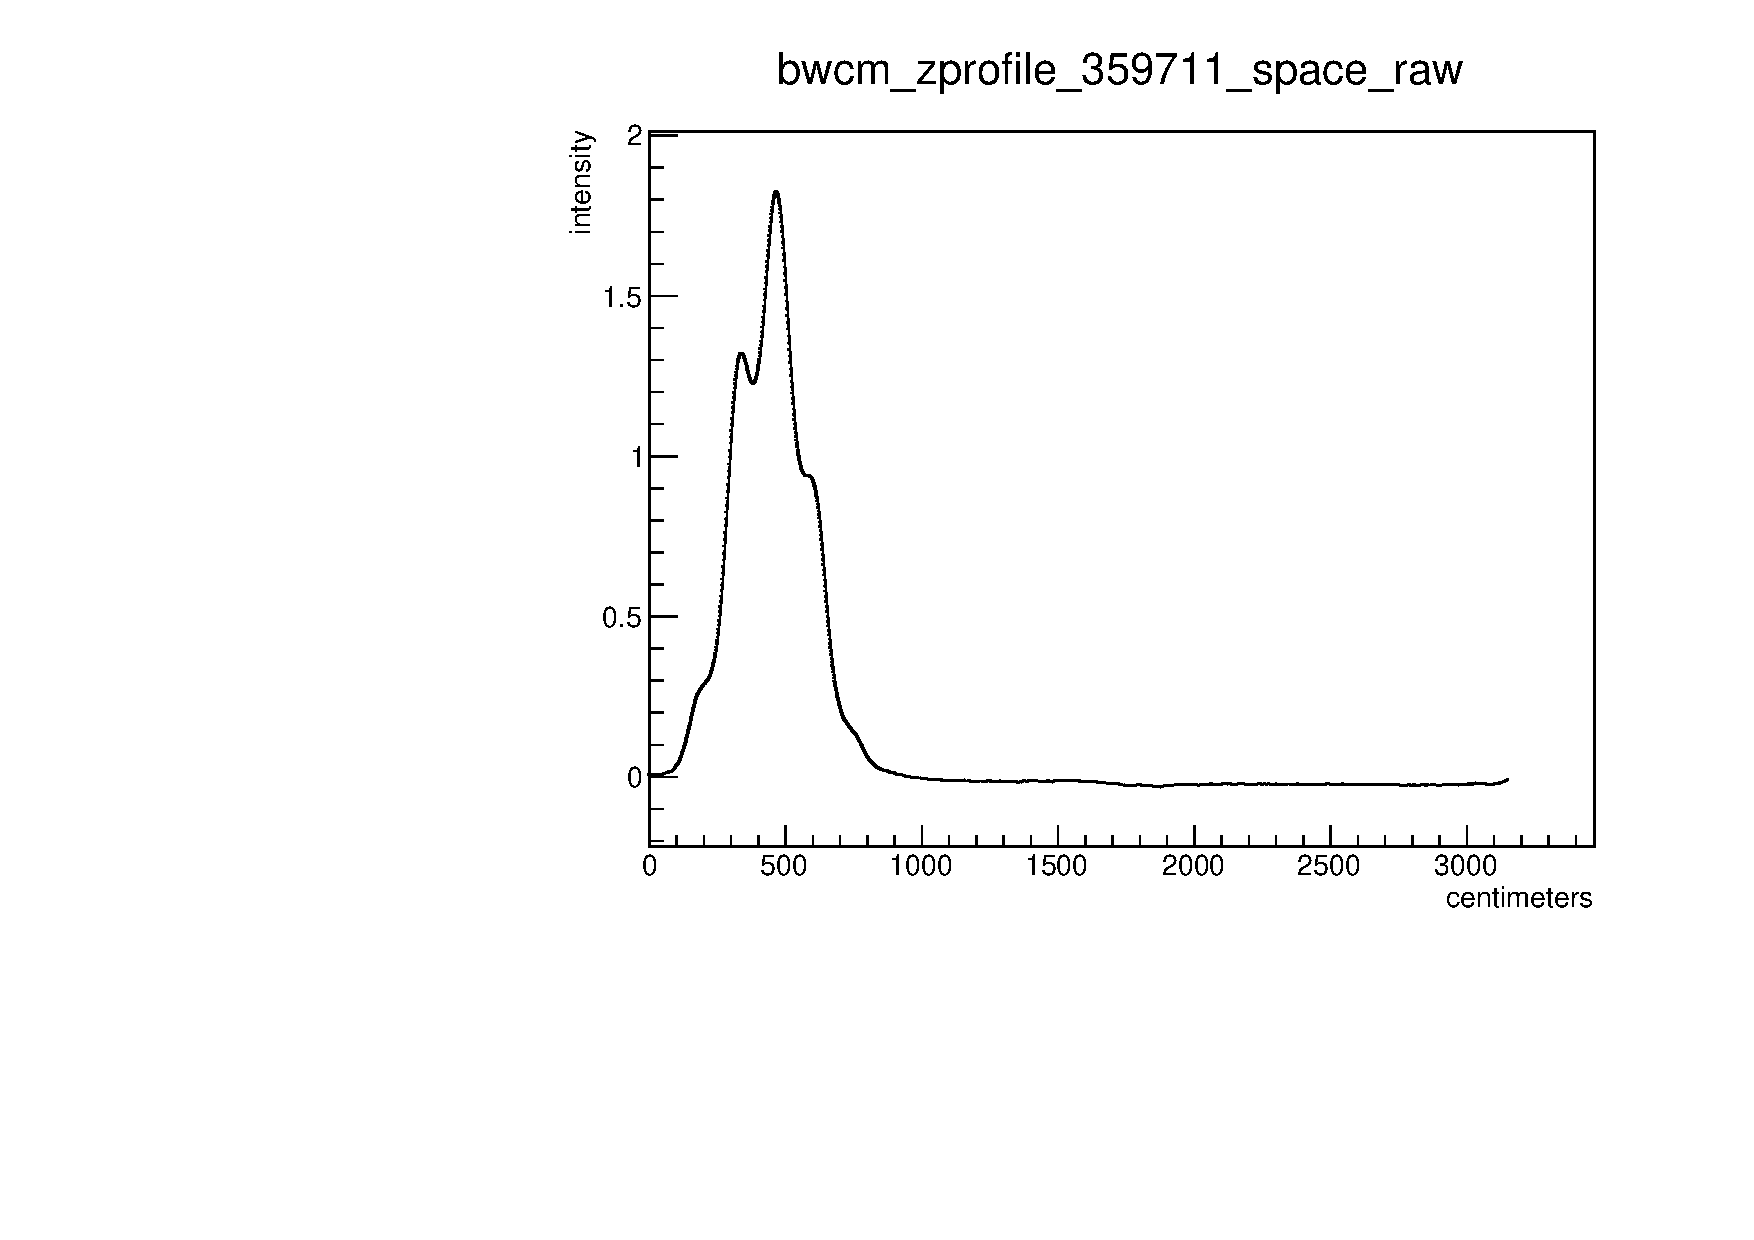
\includegraphics[width=0.6\linewidth]{../ZBunchProfileStudies/figs/bwcm_zprofile_359711_space_raw.pdf}
\end{center}
\caption{Full bunch profile over time period of approximately 106 ns}
\label{fig:bwcm_zprofile_359711_space_raw}
\end{figure}
\end{frame}

\begin{frame}{The Z Bunch Profile}
Shift the profile:
\begin{figure}
\begin{center}
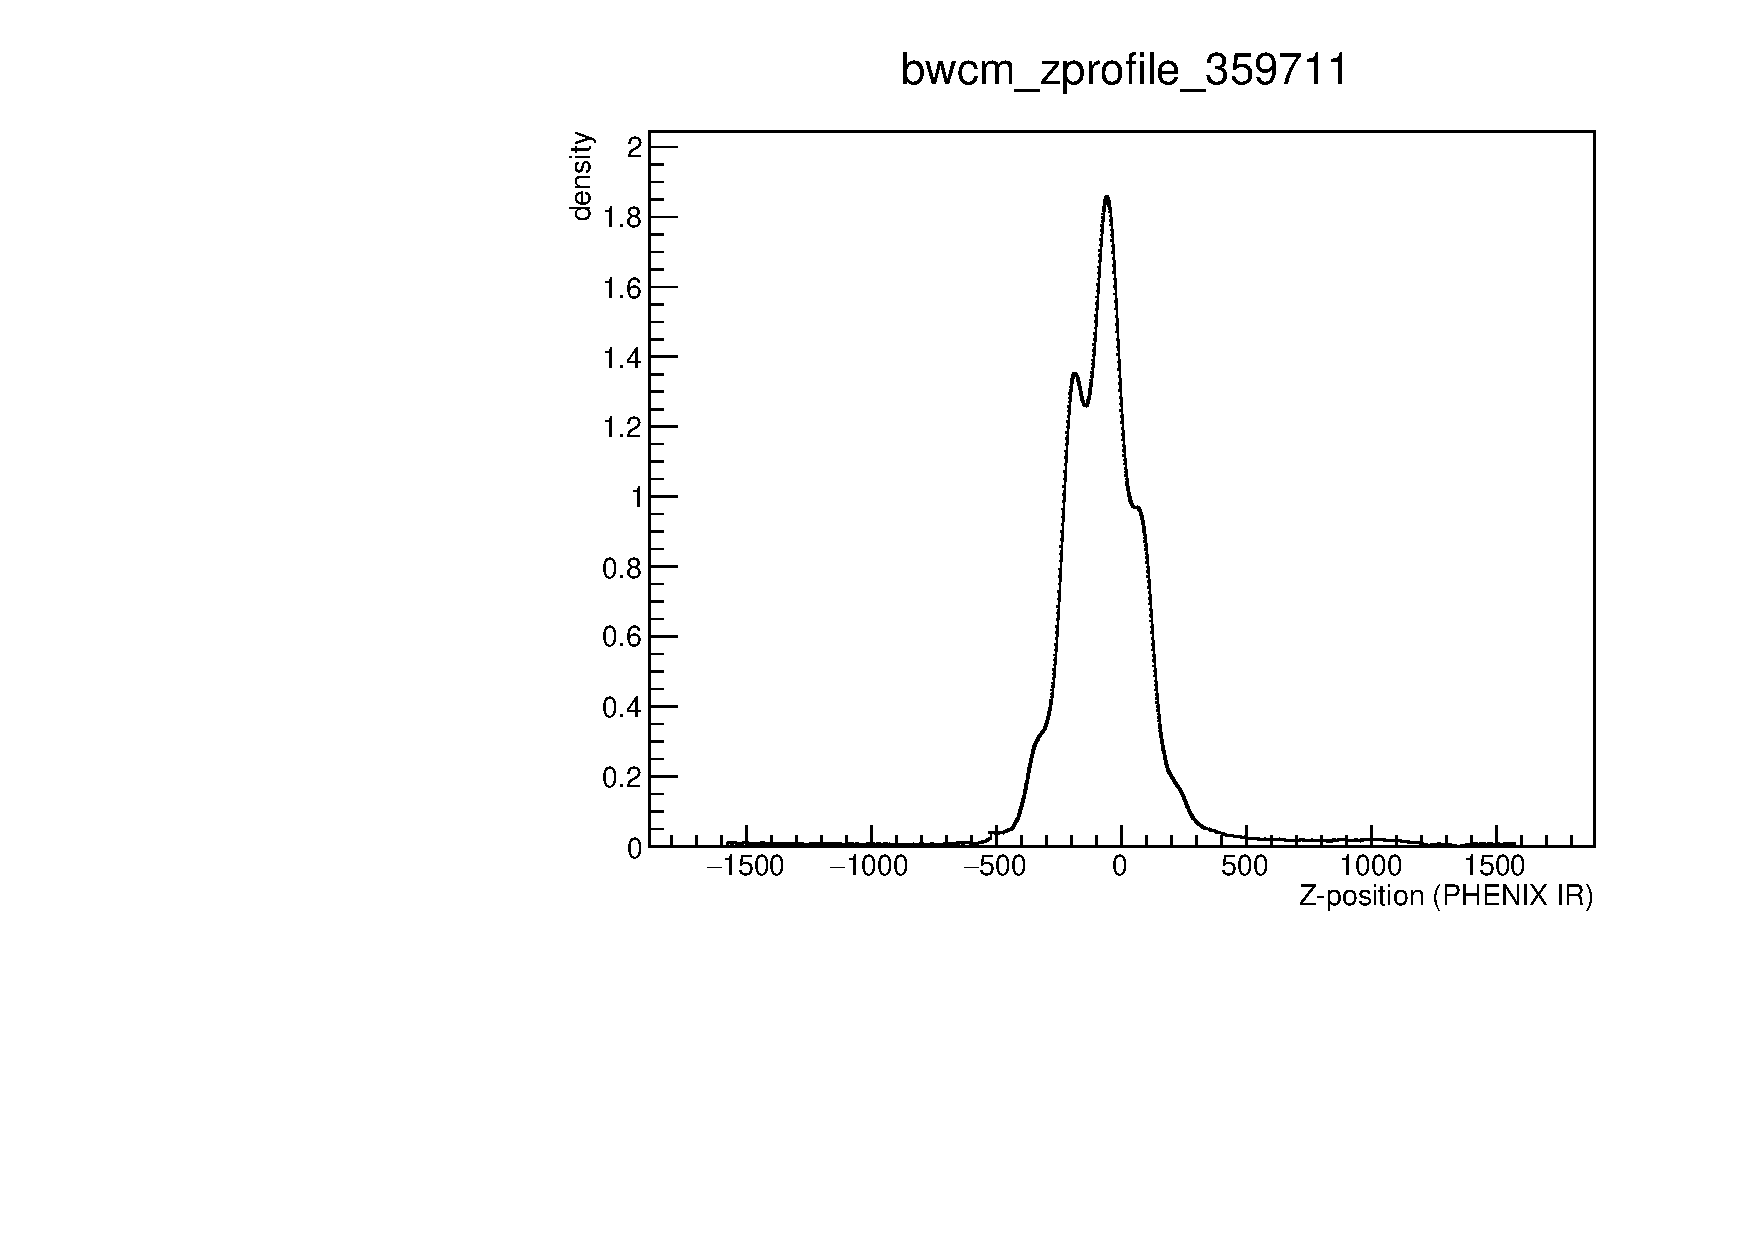
\includegraphics[width=0.6\linewidth]{../ZBunchProfileStudies/figs/bwcm_zprofile_359711_shifted.pdf}
\end{center}
\caption{Full bunch profile over time period of approximately 106 ns, shifted}
\label{fig:bwcm_zprofile_359711_shifted}
\end{figure}
\end{frame}

\begin{frame}{The Z Bunch Profile}
And normalize:
\begin{figure}
\begin{center}
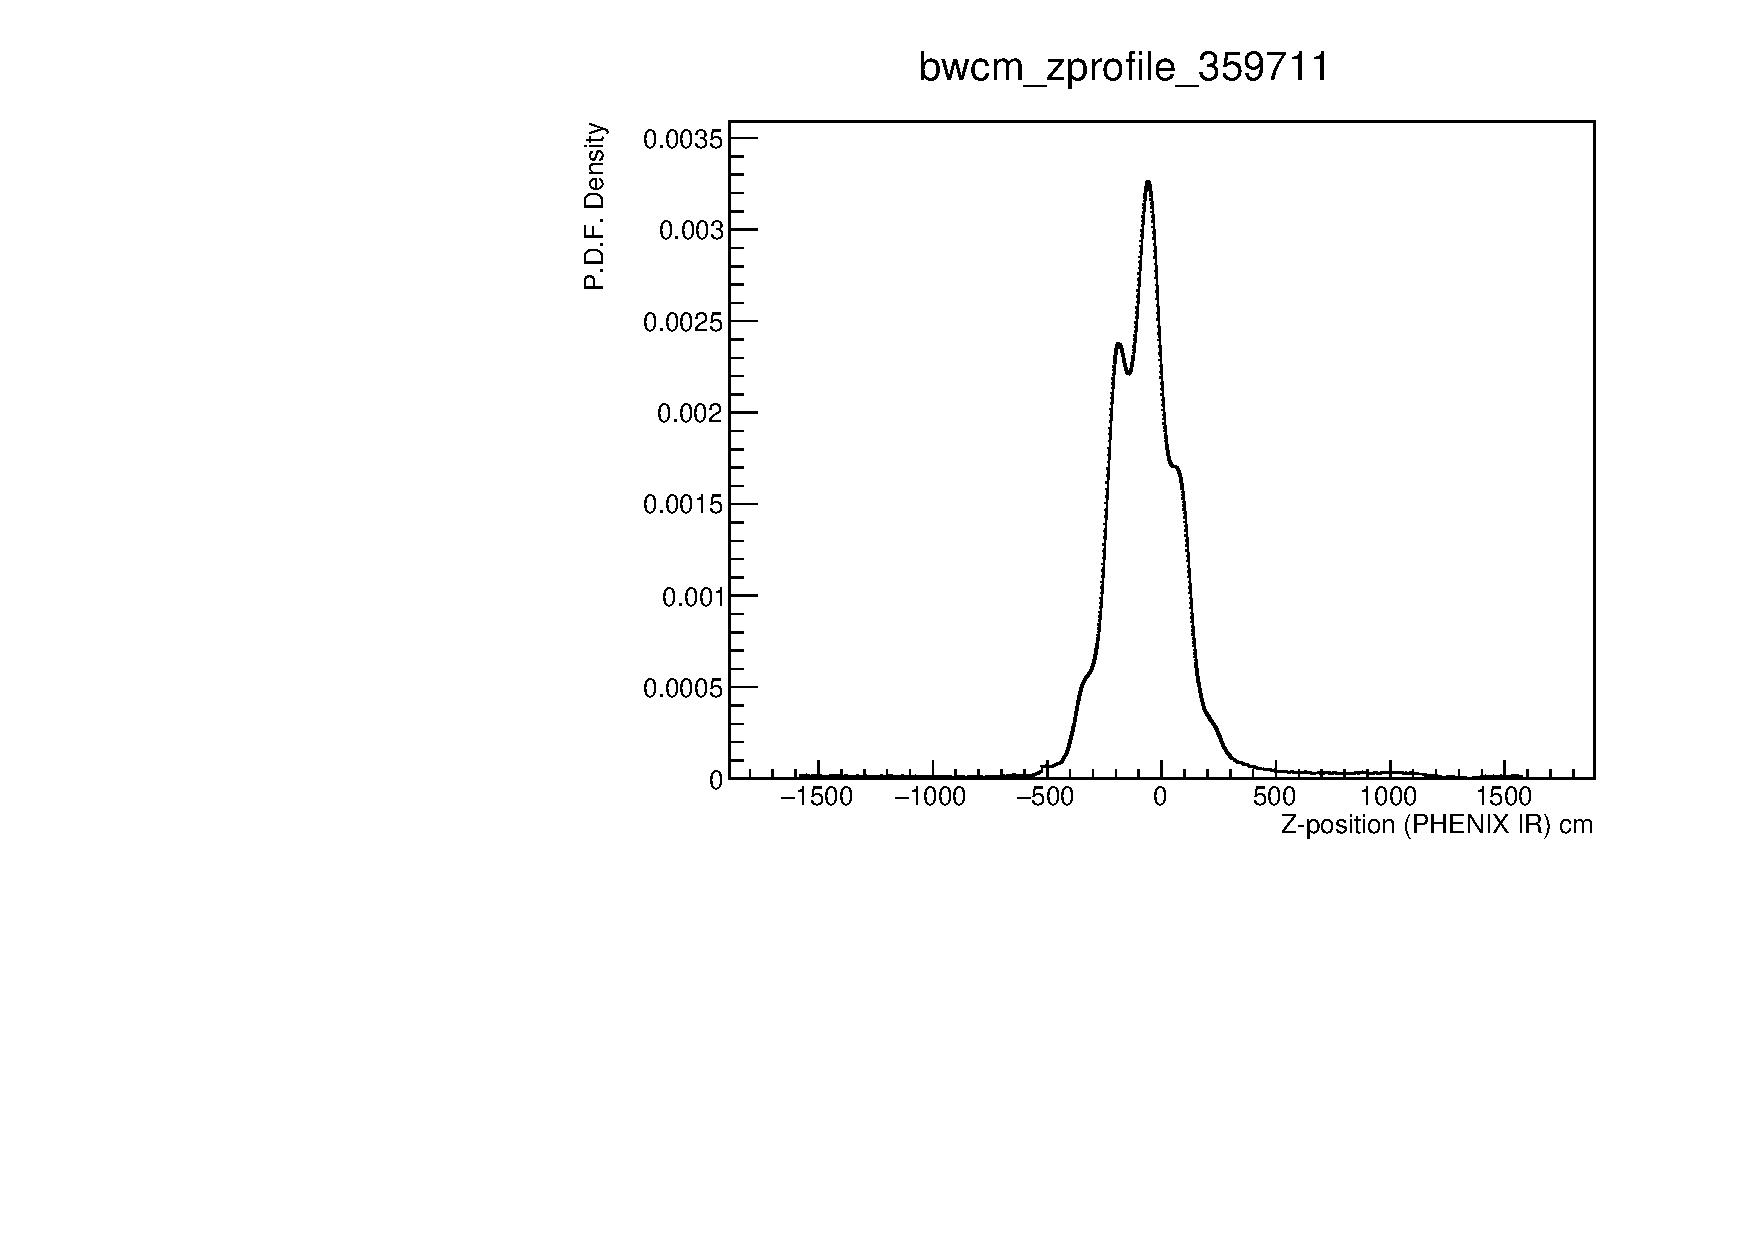
\includegraphics[width=0.6\linewidth]{../ZBunchProfileStudies/figs/bwcm_zprofile_359711_density.pdf}
\end{center}
\caption{Full bunch profile over time period of approximately 106 ns, shifted, normalized}
\label{fig:bwcm_zprofile_359711_density}
\end{figure}
\end{frame}

\begin{frame}{Z Bunch Profile - Inidivdual Bunches, Fill 16444}
\begin{figure}
\begin{center}
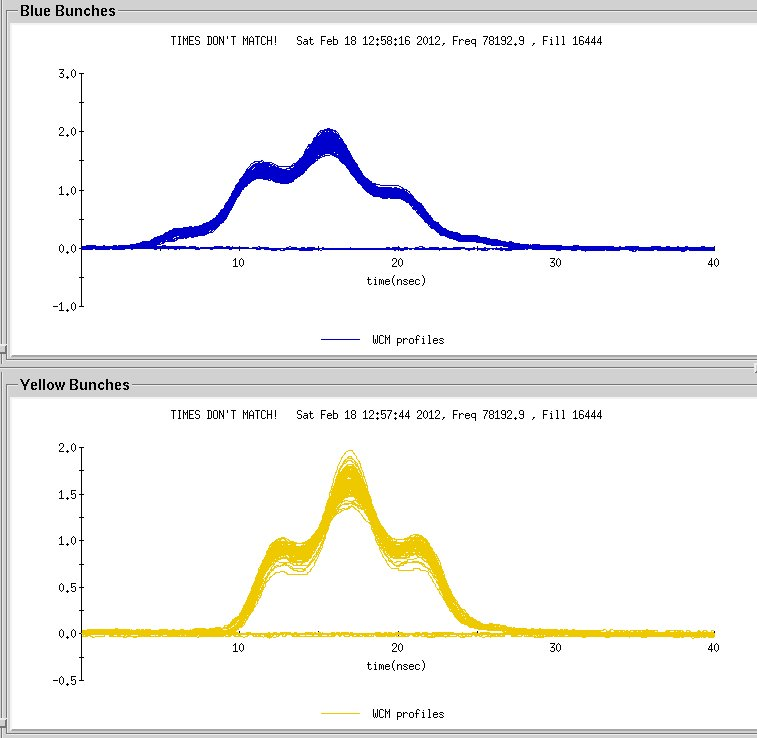
\includegraphics[width=0.5\linewidth]{../ZBunchProfileStudies/figs/wcm_16444.jpeg}
\end{center}
\caption{ }
\label{fig:wcm_16444}
\end{figure}
\end{frame}

\begin{frame}{Z Bunch Profile - Inidivdual Bunches, Fill 16470}
\begin{figure}
\begin{center}
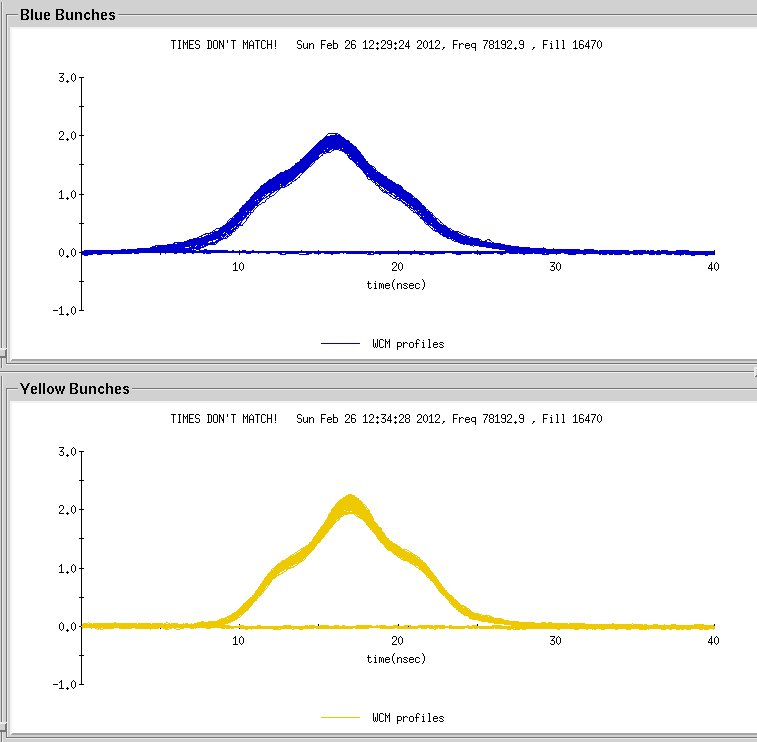
\includegraphics[width=0.5\linewidth]{../ZBunchProfileStudies/figs/wcm_16470.jpeg}
\end{center}
\caption{ Blue (top) and Yellow (bottom) beam profiles for all bunches provided by Angelika Drees from CAD}
\label{fig:wcm_16470}
\end{figure}
\end{frame}

\begin{frame}{Z Bunch Profile - Inidivdual Bunches, Fill 16514}
\begin{figure}
\begin{center}
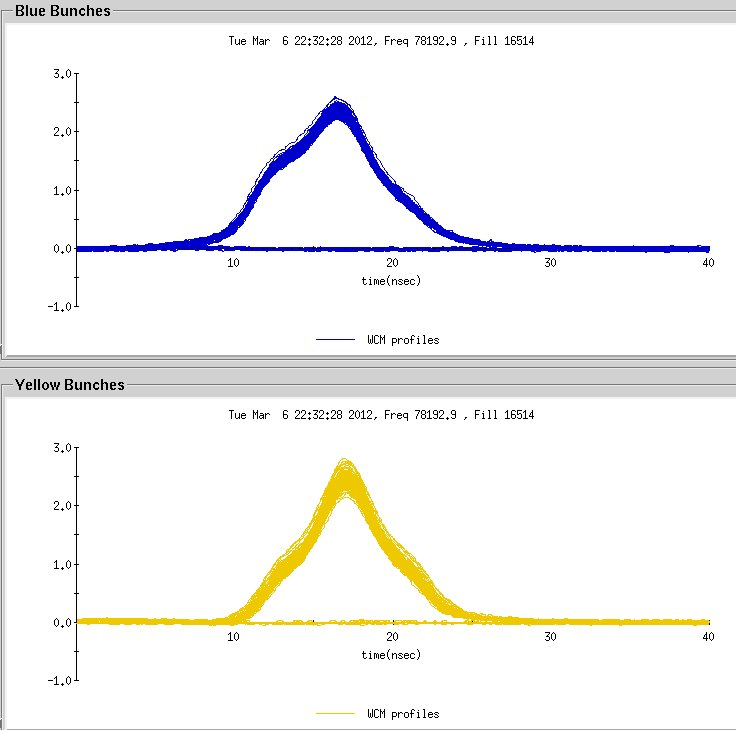
\includegraphics[width=0.5\linewidth]{../ZBunchProfileStudies/figs/wcm_16514.jpeg}
\end{center}
\caption{ Fill 16514, Blue (top) and Yellow (bottom) beam profiles for all bunches provided by Angelika Drees from CAD}
\label{fig:wcm_16514}
\end{figure}
\end{frame}

\begin{frame}{Z Bunch Profile - Inidivdual Bunches, Fill 16587}
\begin{figure}
\begin{center}
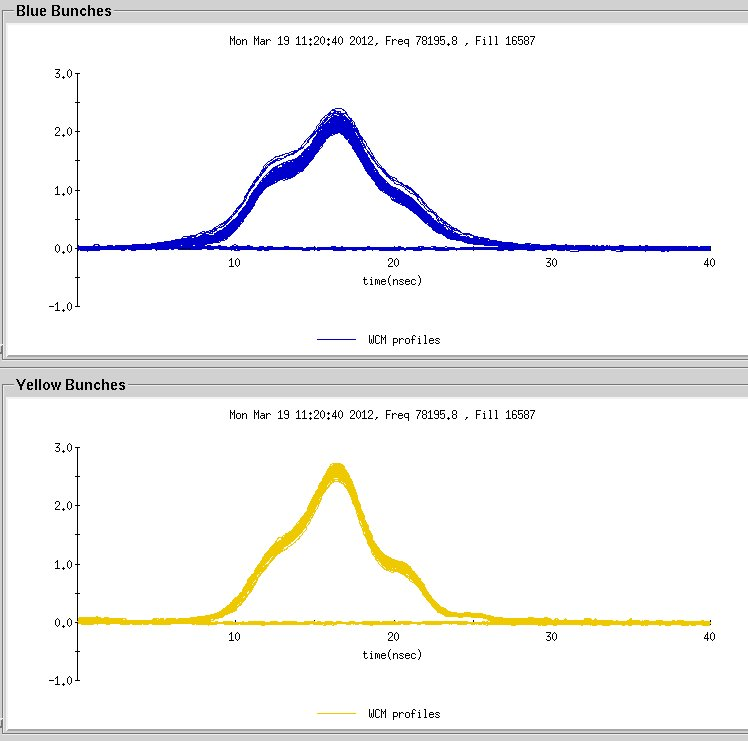
\includegraphics[width=0.5\linewidth]{../ZBunchProfileStudies/figs/wcm_16587.jpeg}
\end{center}
\caption{ Fill 16587 Blue (top) and Yellow (bottom) beam profiles for all bunches provided by Angelika Drees from CAD}
\label{fig:wcm_16587}
\end{figure}
\end{frame}

\begin{frame}{Z Bunch Profile - Inidivdual Bunches, Fill 16625}
\begin{figure}
\begin{center}
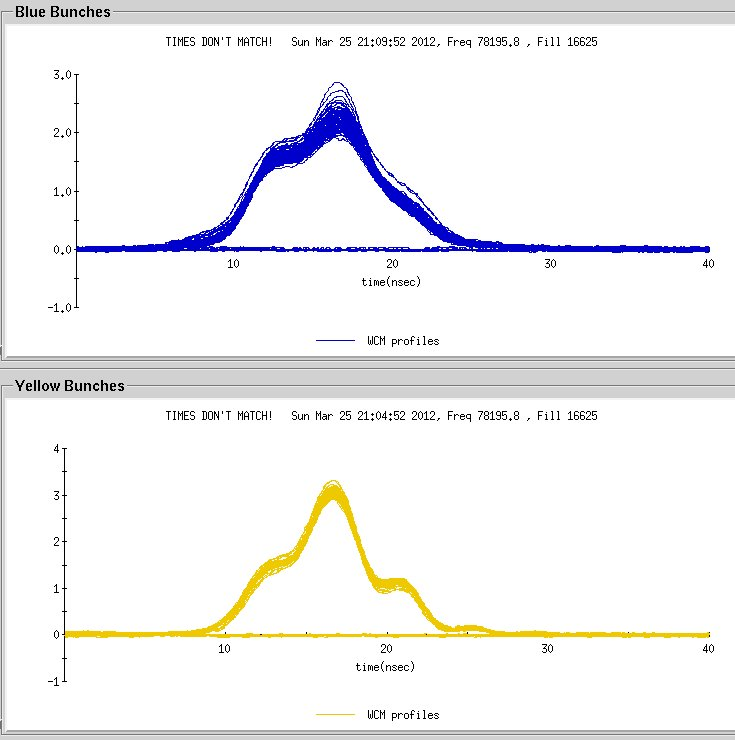
\includegraphics[width=0.5\linewidth]{../ZBunchProfileStudies/figs/wcm_16625.jpeg}
\end{center}
\caption{ Fill 16625, Blue (top) and Yellow (bottom) beam profiles for all bunches provided by Angelika Drees from CAD}
\label{fig:wcm_16625}
\end{figure}
\end{frame}

\begin{frame}{Z Bunch Profile - Inidivdual Bunches, Fill 16655}
\begin{figure}
\begin{center}
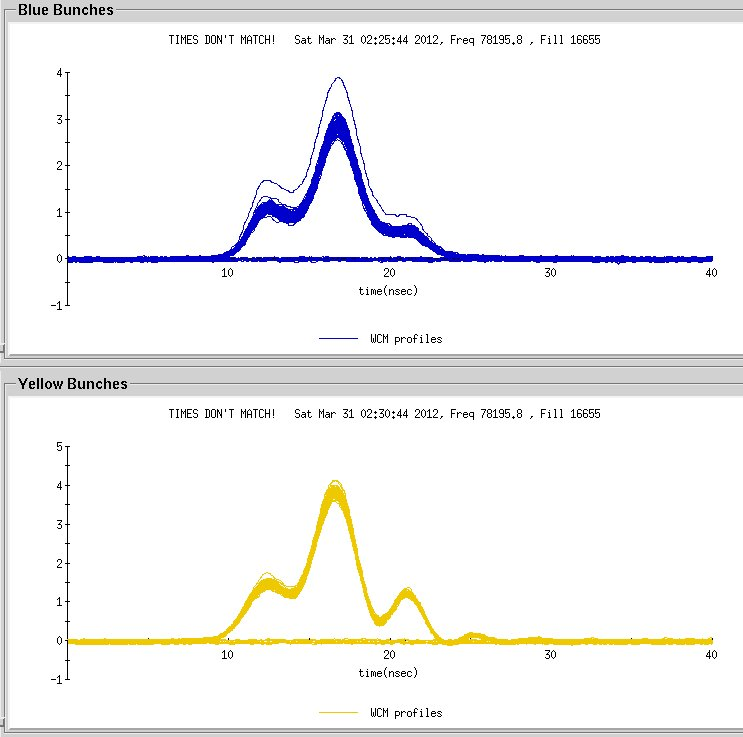
\includegraphics[width=0.5\linewidth]{../ZBunchProfileStudies/figs/wcm_16655.jpeg}
\end{center}
\caption{ Fill 16655, Blue (top) and Yellow (bottom) beam profiles for all bunches provided by Angelika Drees from CAD}
\label{fig:wcm_16655}
\end{figure}
\end{frame}

\begin{frame}{Z Bunch Profile - Inidivdual Bunches, Fill 16671}
\begin{figure}
\begin{center}
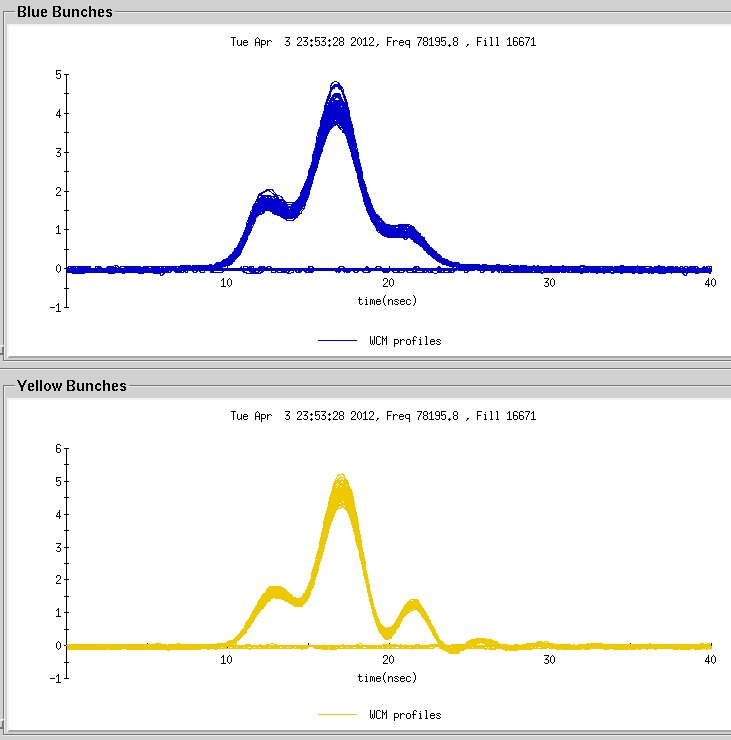
\includegraphics[width=0.5\linewidth]{../ZBunchProfileStudies/figs/wcm_16671.jpeg}
\end{center}
\caption{ Fill 16671, Blue (top) and Yellow (bottom) beam profiles for all bunches provided by Angelika Drees from CAD}
\label{fig:wcm_16671}
\end{figure}
\end{frame}
